\subsection{Directional controller}
The purpose of the directional controller is to have the vehicle turn according to a reference, which the controller receives from the route control, see \secref{Finalprototype}. The design will start out with a proportional controller for the directional controller.
%
\subsubsection{Proportional controller}
A proportional controller implemented in the directional model, see \secref{sec:SteeringModel}, can be seen in \figref{fig:PconAngpic}.
%
\begin{figure}[H]
  \centering
  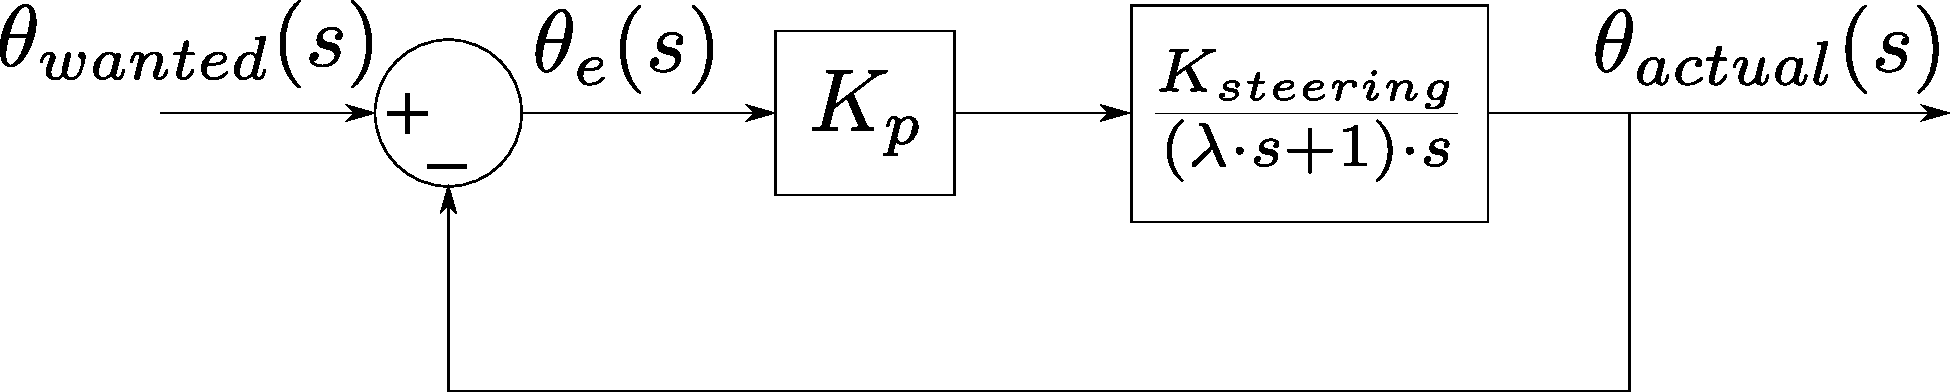
\includegraphics[scale=0.7]{figures/angularController.pdf}
  \caption{Illustration of a proportional controller for the directional steering.}
  \label{fig:PconAngpic}
\end{figure}
%
This will yield the following closed loop transfer function:
%
\begin{flalign}
  \eq{ \frac{\theta_{actual}}{\theta_{wanted}} }{ \frac{\frac{ K_p \cdot K_v \cdot K_s }{ (\lambda \cdot s + 1) \cdot s } }{ \frac{ K_p \cdot K_v \cdot K_s }{ (\lambda \cdot s + 1) \cdot s } + 1} }&\label{eq:PconAng}
\end{flalign}
%
According to \appref{app:steeringGainTest}, the values of $K_s$ and $K_v$ are not needed independently. they are therefore combined to the steering gain, \si{K_{steering}}. From \appref{app:steeringGainTest}, the steering gain can be calculated, with \eqref{eq:PconAng10}.
%
\begin{flalign}
\eq{K_{steering}}{0,3 \cdot v - 0,034}
\label{eq:PconAng10}
\end{flalign}
%
As $v$ is the wanted velocity, which is 1,4 $m \cdot s^{-1}$, $K_{steering}$ is equal to 0,386. And with lambda equal to the servo duty cycle time constant on 30 ms \secref{Servo}, the transfer function yields:
%
\begin{flalign}
  \eq{ \frac{\theta_{actual}}{\theta_{wanted}} }{ \frac{\frac{ K_p \cdot 0,386 }{ (0,03 \cdot s + 1) \cdot s } }{ \frac{ K_p \cdot 0,386 }{ (0,03 \cdot s + 1) \cdot s } + 1} \Rightarrow \frac{1}{\frac{ 0,03 \cdot s^2 + s }{ K_p \cdot 0,386 } + 1}  }&\label{eq:PconAng2}
\end{flalign}
%
From the test done in \appref{app:LinearAreaKp}, it is know, that the steering gain is not constant for different $K_p$ values. The test illustrates a linear area occurs between a $K_p$ value of 1,5 and 3, where the steering gain is constant if the velocity is kept the same. From \eqref{eq:PconAng2}, it can be seen that the time constant will decrease, if the $K_p$ increases. To get the fastest reacting system, with this limitation, $K_p$ is set to be 3. This give a transfer function which yields:
%
\begin{flalign}
  \eq{ \frac{\theta_{actual}}{\theta_{wanted}} }{ \frac{1}{\frac{ 0,03 \cdot s^2 + s }{ 3 \cdot 0,386 } + 1} \Rightarrow \frac{1}{ 0,026 \cdot s^2 + 0,86 \cdot s + 1} }&\label{eq:PconAng4}
\end{flalign}
%
From this transfer function, it can be seen that the gain is equal to one and the system is a second order system. The reason that the proportional controller yields a gain equal to 1, unlike the proportional controller for the velocity, is that there is a integrator in this system, that removes the steady state error. A proportional controller will therefore be sufficient in handling the control the vehicle's angular movement. 
%
The proportional controller is then implemented and tested. For the feedback, the magnetometer from \secref{sec:magnetoSensor} is used. The sampling time for the magnetometer, have been chosen to be the same as the length of the duty cycle for servo, on 30 ms. As the magnetometer only needs to update one time, each time the controller sends a new duty cycle to the servo, there is not needed for a higher sampling frequency. The sampling frequency will then be on:
%
\begin{flalign}
  \eq{ f_{sampling} }{ \frac{1}{30 ms} \Rightarrow 33,33}\unit{Hz} \label{eq:PconAng5}
\end{flalign}
%
The angular controller is then tested, where the start heading is \si{5^{\circ}} and the reference heading is set to \si{45^{\circ}}. The data from the test is illustrated in \figref{fig:AngularTestSim}.
%
\begin{figure}[H]
 	\centering
 	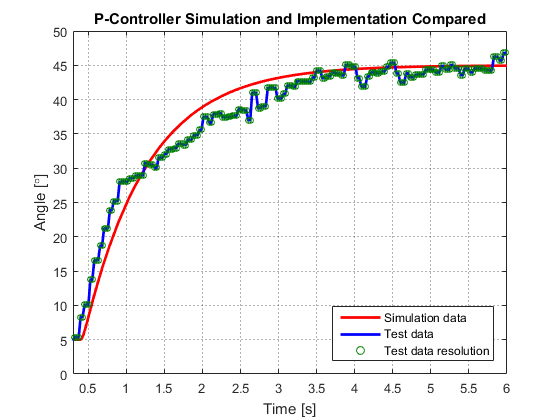
\includegraphics[scale=1]{figures/SteeringAngularTest.png}
 	\caption{Test of the proportional controller, with a start heading on \si{5^{\circ}} and a reference on \si{45^{\circ}}.}
 	\label{fig:AngularTestSim}
\end{figure}
%
As illustrated in \figref{fig:AngularTestSim}, the system looks similar as the simulation, with the same rise and settling time. The proportional controller is thereby utilized in the system, as it functions inside the area where the system is linear and is stable.

The directional controller is designed, and it is thereby possible to design the the distance controller which is around the directional controller.